%%%%%%%%%%%%%%%%%%%%%%%%%%%%%%%%%%%%%%%%%%%%%%%%%%%%
%%% Compilation: PDFLaTeX BibTeX PDFLaTeX PDFLaTeX
%%% Dissertation: Master file                
%%% Style sheet: Antonio Machicao y Priemer   2019.10.05                                   
%%%%%%%%%%%%%%%%%%%%%%%%%%%%%%%%%%%%%%%%%%%%%%%%%%%%

%% based on lsp-skeleton.tex

\documentclass[
a4paper,
11pt,
twoside,	% oneside, twoside
%twoside=false, 	%No difference between left and right page
openright,	% openleft, openright, openany
BCOR=12mm,	% Correcting the bind margin
%DIV=calc,	% Correcting Satzspiegel + DIV=last in localpackages
]{scrbook}

%% Cf. localpackages for further page settings


%% For a faster compilation use option: ``draft''
%\documentclass[draft,a4paper,12pt]{scrbook}

\setcounter{tocdepth}{4}
\setcounter{secnumdepth}{3}


%%%%%%%%%%%%%%%%%%%%%%%%%%%%%%%%%%
%%%  PACKAGES METADATA COMMANDS HYPHENATION            
%%%%%%%%%%%%%%%%%%%%%%%%%%%%%%%%%%

% put all additional commands you need in the 
% following files. If you do not know what this might 
% mean, you can safely ignore this section

%%%%%%%%%%%%%%%%%%%%%%%%%%%%%%%%%%%%%%%%%%%%%%%%%%%%
%%%          MyP-Packages   2020.11.12   PhD thesis + PDFLaTeX
%%%%%%%%%%%%%%%%%%%%%%%%%%%%%%%%%%%%%%%%%%%%%%%%%%%%


\usepackage[utf8]{inputenc}

%%% Text in German:
%\usepackage[english,ngerman]{babel}

%% Text in English:
\usepackage[ngerman,english]{babel}

	%%% Change "Bibliography" into "References"
	\addto{\captionsenglish}{\renewcommand{\bibname}{References}}

	%\addto{\captionsenglish}{\renewcommand{\bibname}{Literatur}}
	
	%%% Change ''Abbildung'' into ''Abb.'' (for: babel)
	%\renewcommand{\thefigure}{\arabic{figure}}
	%\addto\captionsngerman{%
	%	\renewcommand{\figurename}{Abb.}%
	%}
	%\renewcommand{\figurename}{Abb.} 

	
%% TIPA encoding needs T3 & T1
\usepackage[T3,T1]{fontenc}

%% Fonts
%\usepackage{lmodern}

\usepackage{libertine}
	% change typewriter font to lmodern (smaller than tt in libertine)
	\renewcommand\ttdefault{lmtt}
	

%% For compatible mathematics (PDFLaTeX), it is recommended to use 
%\usepackage[libertine]{newtxmath}

%% Blind text: \blindtext \Blindtext \blindtext[5] \blindlist{itemize}[x] ...
\usepackage{blindtext}

%% ulem: Strike out
\usepackage[normalem]{ulem}  

%% graphicx: if gb4e is active PDFLaTeX does not accept files with underscore. PDFLaTeX only accepts files with .jpg, .png, .pdf endings
\usepackage{graphicx}


%%%%%%%%%%%%%%%%%%%%%%%%%%%%%%%%
%%%           Special Math-Symbols                   
%%%%%%%%%%%%%%%%%%%%%%%%%%%%%%%%

\usepackage{amsmath}
\usepackage{amsfonts}
\usepackage{amssymb}
\usepackage{MnSymbol}            %% Meaning brackets

\usepackage{pifont}                   %% checkmark

\usepackage{wasysym}              %% \Square \XBox \CheckedBox


%%%%%%%%%%%%%%%%%%%%%%%%%%%%%%%%
%%%         Tables & Lists & Columns            
%%%%%%%%%%%%%%%%%%%%%%%%%%%%%%%%

% Text in columns: \begin{multicols}{n} \columnbreak \end{multicols}
\usepackage{multicol}
%	\setlength{\columnsep}{.5cm}	

%% Tables with specified width
\usepackage{tabularx}

%% For complex tables
\usepackage{array}

%% For other tables
\usepackage{booktabs}

%% For more than one row in a table
\usepackage{multirow}

%% Special lists: itemize*
\usepackage{mdwlist}


%%%%%%%%%%%%%%%%%%%%%%%%%%%%%%%%
%%%          Coloured elements                  
%%%%%%%%%%%%%%%%%%%%%%%%%%%%%%%%
%Use xcolor before `gb4e'!
\usepackage{xcolor}


%%%%%%%%%%%%%%%%%%%%%%%%%%%%%%%%
%%%         TikZ                               
%%%%%%%%%%%%%%%%%%%%%%%%%%%%%%%%
% 
\usepackage{tikz}
\usetikzlibrary{patterns}


%%%%%%%%%%%%%%%%%%%%%%%%%%%%%%%%
%%%          Trees                               
%%%%%%%%%%%%%%%%%%%%%%%%%%%%%%%%
%% Forest must be loaded before `gb4e'
%% Package loaded with forest: tikz

\usepackage{forest}
	%% Needed for the "actual forest version"
	\useforestlibrary{linguistics}
	\forestapplylibrarydefaults{linguistics}



%%%%%%%%%%%%%%%%%%%%%%%%%%%%%%%%
%%%%       Attribute Value Matrices               
%%%%%%%%%%%%%%%%%%%%%%%%%%%%%%%%
\usepackage{langsci-avm}


%%%%%%%%%%%%%%%%%%%%%%%%%%%%%%%%
%%%          IPA                                 
%%%%%%%%%%%%%%%%%%%%%%%%%%%%%%%%
\usepackage[noenc,safe]{tipa}	


%%%%%%%%%%%%%%%%%%%%%%%%%%%%%%%%
%%%%          Verbatim                            
%%%%%%%%%%%%%%%%%%%%%%%%%%%%%%%%
%%`Listings' must be loaded before `gb4e', use `verbatim' otherwise
\usepackage{listings}

	\lstset{
		language=TeX,
		backgroundcolor=\color{lightgray},
		basicstyle={\footnotesize\ttfamily\color{blue}},
		showstringspaces=false,
		%	showspaces=false,
		breaklines=true,
		%	tabsize=2,
		columns=flexible
	}
	\lstset{literate=%
		{Ö}{{\"O}}1
		{Ä}{{\"A}}1
		{Ü}{{\"U}}1
		{ß}{{\ss}}2
		{ü}{{\"u}}1
		{ä}{{\"a}}1
		{ö}{{\"o}}1
	}
	

%%%%%%%%%%%%%%%%%%%%%%%%%%%%%%%%
%%%          Indices                            
%%%%%%%%%%%%%%%%%%%%%%%%%%%%%%%%

\usepackage{imakeidx}

\usepackage{acronym}


%%%%%%%%%%%%%%%%%%%%%%%%%%%%%%%%
%%%          Bibliography                        
%%%%%%%%%%%%%%%%%%%%%%%%%%%%%%%%

\usepackage[sectionbib]{natbib}
	\setlength{\bibsep}{0mm%pt plus 0.3ex
	}
	\setcitestyle{notesep={:~}}
	\setcitestyle{aysep={}} 


%%%%%%%%%%%%%%%%%%%%%%%%%%%%%%%%
%%%%          Settings of the page                
%%%%%%%%%%%%%%%%%%%%%%%%%%%%%%%%
%
%\KOMAoptions{
%DIV=last,	% Correcting Satzspiegel + DIV=calc in master (DIV=last after font)
%headsepline, 		%Line between heading and text (cf. Package scrpage2)
%}
%
%Headers & Footers
\usepackage[headsepline,
			%footsepline
			]{scrlayer-scrpage}
	\pagestyle{scrheadings}
	\clearscrheadfoot		%Clean all headers & footers
%	%%%%%%%%%%%%%%%%%%%%%%%%%	
%	%%One sided document:
%	%\ihead{Kopfzeile innen}
%	%\chead{Kopfzeile Mitte}
%	\ohead{\headmark}
%	\automark{section}
%	%\ifoot{Fußzeile innen}
%	%\cfoot{Fußzeile Mitte}
%	\ofoot{\pagemark} 
	%%%%%%%%%%%%%%%%%%%%%%%%%
	%%Two sided document:
	%\ihead{Kopfzeile innen}
	%\chead{Kopfzeile Mitte}
	\ohead{\headmark}
	\automark[chapter]{chapter}
	%\ifoot{Fußzeile innen}
	%\cfoot{Fußzeile Mitte}
	\ofoot{\pagemark} 
	%%%%%%%%%%%%%%%%%%%%%%%%%

%% (Vertical) Spacing
\usepackage{setspace}
	\onehalfspacing % to set the line spacing to 1.5. If you require single line spacing, comment this out.

%% Space for abbreviations 'i.d.R'
\usepackage{xspace}


%% Geometry: Setting up margins. This package must be loaded before `gb4e'
%\usepackage{geometry} 
%	\geometry{
%	left=3cm,
%	right=3cm,
%	%vmargin=3cm,
%	top=3cm,
%	bottom=3cm,
%	includeheadfoot
%	}


%% Footnote options: 
%% [bottom]: FN at the bottom, 
%% [hang] + 10pt: FN align
%% [splitrule]: If a FN is split across 2 pages, it adds a full-linelength line (http://tex.stackexchange.com/questions/32208/footnote-runs-onto-second-page)
\usepackage[bottom, hang, splitrule]{footmisc}
	\setlength\footnotemargin{0pt}
%	\setlength{\footnotesep}{.7\baselineskip}	%More spacing btw. FNs


%%%%%%%%%%%%%%%%%%%%%%%%%%%%%%%%%
%%%%%          Margin notes                        
%%%%%%%%%%%%%%%%%%%%%%%%%%%%%%%%%
\usepackage{todonotes}


%%%%%%%%%%%%%%%%%%%%%%%%%%%%%%%%
%%%           Examples                           
%%%%%%%%%%%%%%%%%%%%%%%%%%%%%%%%
\usepackage{langsci-gb4e}


%%%%%%%%%%%%%%%%%%%%%%%%%%%%%%%%
%%%          Hyperref & URL                      
%%%%%%%%%%%%%%%%%%%%%%%%%%%%%%%%
%\usepackage[hyphens]{url}
\usepackage[
bookmarksnumbered, %For numbered bookmarks in PDF
%	hidelinks %For links without colored borders
]{hyperref}

%%%%%%%%%%%%%%%%%%%%%%%%%%%%%%%%%%%%%%%%%%%%%%%%%%%%
%%%          MyP-Metadata   2020.11.12   PhD thesis + PDFLaTeX
%%%%%%%%%%%%%%%%%%%%%%%%%%%%%%%%%%%%%%%%%%%%%%%%%%%%


\title{\begin{Huge}NP-Arguments in NPs\end{Huge}}

\subtitle{An Analysis of German and Spanish Noun Phrases in Head-Driven Phrase Structure Grammar}


\dedication{For NN}

\author{Antonio Machicao y Priemer\\
	\url{http://www.linguistik.hu-berlin.de/staff/amyp}\\
	\href{mailto:mapriema@hu-berlin.de}{mapriema@hu-berlin.de}}


%\date{20/07/2019}


\publishers{Humboldt-Universität zu Berlin}


%% Properties of the PDF
\hypersetup{
	pdftitle={NP-Arguments in NPs},
	%	pdfsubject={Syntax},
	pdfauthor={Antonio Machicao y Priemer},
	pdfkeywords={syntax, semantics, quantifier, DP, NP, German, Spanish}
}

%% hyphenation points for line breaks
%% Normally, automatic hyphenation in LaTeX is very good
%% If a word is mis-hyphenated, add it to this file
%%
%% add information to TeX file before \begin{document} with:
%% %% hyphenation points for line breaks
%% Normally, automatic hyphenation in LaTeX is very good
%% If a word is mis-hyphenated, add it to this file
%%
%% add information to TeX file before \begin{document} with:
%% %% hyphenation points for line breaks
%% Normally, automatic hyphenation in LaTeX is very good
%% If a word is mis-hyphenated, add it to this file
%%
%% add information to TeX file before \begin{document} with:
%% \include{localhyphenation}

\hyphenation{
%%English hyphenation	
	af-fri-cate
	af-fri-cates
	a-na-ly-sis
	a-na-ly-ses
	a-na-ly-se
	a-na-ly-sed
	com-ple-ment
	com-ple-ments
%% German hyphenation
	Ein-füh-rungs-ka-pi-tel
}

\hyphenation{
%%English hyphenation	
	af-fri-cate
	af-fri-cates
	a-na-ly-sis
	a-na-ly-ses
	a-na-ly-se
	a-na-ly-sed
	com-ple-ment
	com-ple-ments
%% German hyphenation
	Ein-füh-rungs-ka-pi-tel
}

\hyphenation{
%%English hyphenation	
	af-fri-cate
	af-fri-cates
	a-na-ly-sis
	a-na-ly-ses
	a-na-ly-se
	a-na-ly-sed
	com-ple-ment
	com-ple-ments
%% German hyphenation
	Ein-füh-rungs-ka-pi-tel
}

%%%%%%%%%%%%%%%%%%%%%%%%%%%%%%%%%%%%%%%%%%%%%%%%%%%%
%%%           MyP-Commands  2019.10.05    PhD thesis + PDF-LaTeX       
%%%%%%%%%%%%%%%%%%%%%%%%%%%%%%%%%%%%%%%%%%%%%%%%%%%%   

%%%%%%%%%%%%%%%%%%%%%%%%%%%%%%%%
%% Extra complex long definitions (e.g. X-bar) are in:
%% 
%%% localextracommands/lec-...

%%%%%%%%%%%%%%%%%%%%%%%%%%%%%%%%
%% ABBREVIATIONS
%%%%%%%%%%%%%%%%%%%%%%%%%%%%%%%%

%%%%%%%%%%%%%%%%%%%%%%%%%%%%%%%%
% Abbreviations in German
% package needed: xspace
% Short space in German abbreviations: \,	

\newcommand{\zB}{\mbox{z.\,B.}\xspace}



%%%%%%%%%%%%%%%%%%%%%%%%%%%%%%%%
%% TYPE SETTING
%%%%%%%%%%%%%%%%%%%%%%%%%%%%%%%%

%%%%%%%%%%%%%%%%%%%%%%%%%%%%%%%%
% German quotation marks:
\newcommand{\gqq}[1]{\glqq{}#1\grqq{}}		%double
\newcommand{\gq}[1]{\glq{}#1\grq{}}			%simple



%%%%%%%%%%%%%%%%%%%%%%%%%%%%%%%%
% Writing text with colour:
% package needed: xcolor
\newcommand{\blue}[1]{\textcolor{blue}{#1}}
\newcommand{\red}[1]{\textcolor{red}{#1}}

%%%%%%%%%%%%%%%%%%%%%%%%%%%%%%%%
%% Marking text with colour: 
%%% package needed: color
\newcommand{\clrr}[1]{\colorbox{red}{#1}}
\newcommand{\clry}[1]{\colorbox{yellow}{#1}}


%%%%%%%%%%%%%%%%%%%%%%%%%%%%%%%%
%% LINGUISTIC TYPOGRAPHY
%%%%%%%%%%%%%%%%%%%%%%%%%%%%%%%%



%%%%%%%%%%%%%%%%%%%%%%%%%%%%%%%%
%% Semantic types (<e,t>), features, variables and graphemes in angled brackets 

%%% types and variables, in math mode: angled brackets + italics + no space
%\newcommand{\type}[1]{$<#1>$}

%%% OR more correctly: 
%%% Types and Variables: chevrons! + text in math mode (italics + no space)
\newcommand{\type}[1]{$\langle #1 \rangle$} %% In Math Mode, only single types
\newcommand{\typem}[1]{\langle #1 \rangle } %% Mathmode extra, complex types

%%% Features and Graphemes: chevrons! + normal font
\newcommand{\ab}[1]{$\langle$#1$\rangle$} %% no italics
\newcommand{\abe}[1]{$\langle$\emph{#1}$\rangle$} %% italics

%%% Meaning brackets ([[xyz]]) + expression in italics
%% package needed: MnSymbol
\newcommand{\sem}[1]{$\lsem$\emph{#1}$\rsem$} %% italics
\newcommand{\semm}[1]{\lsem \textrm{\emph{#1}} \rsem} %% in math mode, italics

%% Denotational set
%% use in math mode: \ds{\typem{e,t}}
\newcommand{\ds}[1]{\textrm{D}_{#1}}

%% Predicates in formulae
%% use in math mode: \pred{Tisch} 
%\newcommand{\pred}[1]{\textrm{#1}'}  %% simple predicate with prime
\newcommand{\pred}[1]{\texttt{#1}}  %% simple predicate in type writer
\newcommand{\predO}[1]{\textrm{\textsc{#1}}} %% Operator in small caps

%% Presuppositions
\newcommand{\prspp}{$\gg$} 

%% Implicature
\newcommand{\implc}{$+ \mkern-5mu >$} 

%%%%%%%%%%%%%%%%%%%%%%%%%%%%%%%%
%% Function symbol in Beamer Class!
%% italics and serif
\newcommand{\func}{\emph{\textrm{f}}}
\newcommand{\gunc}{\emph{\textrm{g}}}
\newcommand{\chiF}[1]{\chi _{\textrm{#1}}} 

%%%%%%%%%%%%%%%%%%%%%%%%%%%%%%%%
%% HPSG: Features and Values!
\newcommand{\wert}[1]{\emph{#1}}        %Values & Types
\newcommand{\feat}[1]{\textsc{#1}}       %Features
\newcommand{\inx}[1]{\fbox{\footnotesize #1}}       %HPSG indices

%%%%%%%%%%%%%%%%%%%%%%%%%%%%%%%%
%% Subscript & Superscript: no italics inside math mode
\newcommand{\down}[1]{\textsubscript{#1}}
\newcommand{\downm}[1]{_{\textrm{#1}}}

\newcommand{\up}[1]{\textsuperscript{#1}}
\newcommand{\upm}[1]{^{\textrm{#1}}}

%%%%%%%%%%%%%%%%%%%%%%%%%%%%%%%%%
%% Shorter Underline
\DeclareTextCommand{\_}{T1}{\leavevmode \kern.06em\vbox{\hrule width.4em}}

%%%%%%%%%%%%%%%%%%%%%%%%%%%%%%%%
%% (Syntactic) Trees
% package needed: forest
% with option: linguistics

%%% Setting for complex trees
%% "bottom word" is the old "sn edges", but the later is used as default (idk y)
\forestset{
	bottom word/.style={for tree={parent anchor=south, child anchor=north,align=center,base=bottom,where n children=0{tier=word,inner xsep=0pt,outer sep=0pt}{}}}, 
	%
	background tree/.style={for tree={text opacity=0.2,draw opacity=0.2,edge={draw opacity=0.2}}}
}

%% Use HideWd for translations when using roof and the translations are longer than the original text
%% https://tex.stackexchange.com/questions/167978/smaller-roofs-for-forest
\newcommand\HideWd[1]{%
	\makebox[0pt]{#1}%
}



%%%%%%%%%%%%%%%%%%%%%%%%%%%%%%%%
%% NOTES & BOX
%%%%%%%%%%%%%%%%%%%%%%%%%%%%%%%%

%%%%%%%%%%%%%%%%%%%%%%%%%%%%%%%%
%% Outputbox
\newcommand{\outputbox}[1]{\noindent\fbox{\parbox[t][][t]{0.98\linewidth}{#1}}\vspace{0.5em}}

%%%%%%%%%%%%%%%%%%%%%%%%%%%%%%%%
%% TO DO NOTES
% package needed: todonote
\newcommand{\todolit}[1]{\todo[color=green!40]{LIT: #1}}
\newcommand{\todored}[1]{\todo[color=red!60]{#1}}


%%%%%%%%%%%%%%%%%%%%%%%%%%%%%%%%
%% Chapter Notes: \begin{chnote}\end{chnote}
%%% package needed: 
%
\newenvironment{chnote}{
	\color{blue}
	%	\noindent \paragraph*{CHAPTER NOTES} 
	\begin{itemize*}
	}
	%	
	{
	\end{itemize*} 
}


%%%%%%%%%%%%%%%%%%%%%%%%%%%%%%%%
%% Index newcommand:
%%% package needed: imakeidx package
\newcommand{\is}[1]{\index{#1}{#1}}

%for terms of implementations (files, code, etc.)
\newcommand{\ist}[1]{\index{#1}{\texttt{#1}}}

%for terms in math mode
\newcommand{\ism}[1]{\index{$#1$}{$#1$}}   


%%%%%%%%%%%%%%%%%%%%%%%%%%%%%%%%
%% Theoretical Abbreviations & Commands
%% in English: 

%%%% Theories
\newcommand{\GB}{\index{Government \& Binding Theory (GB)}{GB}}	

\newcommand{\GPSG}{\index{Generalized Phrase Structure Grammar (GPSG)}{\ac{GPSG}}}	

%%%% HPSG Terminology & Commands
\newcommand{\attr}[1]{\index{attribute!\textsc{#1}}{\textsc{#1}}}
	

%%%% HPSG Principles:
\newcommand{\CaseP}{\index{principle!Case Principle (CaseP)}{CaseP}}


%%%% Further Terminology & Commands
\newcommand{\throle}{\index{theta role}{theta role}}
\newcommand{\throles}{\index{theta role}{theta roles}}


%%%%%%%%%%%%%%%%%%%%%%%%%%%%%%%%
%% Corpora
% 
\newcommand{\ESCOW}{\citetext{ESCOW \citeyear{SchaeferR&Co12a}}}

\makeindex


%%%%%%%%%%%%%%%%%%%%%%%%%%%%%%%%%%
%%%             PREAMBLE'S END                  
%%%%%%%%%%%%%%%%%%%%%%%%%%%%%%%%%%

\begin{document}       


%%%%%%%%%%%%%%%%%%%%%%%%%%%%%%%%%%
%%%     FRONTMATTER
%%%%%%%%%%%%%%%%%%%%%%%%%%%%%%%%%%


%%% FRONTPAGE: Use ch000-Frontpage OR use maketitle 
%%%%%%%%%%%%%%%%%%%%%%%%%%%%%%%%%%%%%%%%%%%%%%%%%
%% Compile the master file
%% this file contains the frontpage only
%% Template for theis (Antonio Machicao y Priemer)
%%%%%%%%%%%%%%%%%%%%%%%%%%%%%%%%%%%%%%%%%%%%%%%%%


\thispagestyle{empty}


\vspace{5.6cm}

%% complete page centered
\begin{center}

%% Title
\begin{minipage}{.99\textwidth}
	\begin{center}

	\begin{huge}
	\textbf{NP-Arguments in NPs}
	\end{huge}

	\end{center}
\end{minipage}


\vspace{.5cm}

%% Subtitle
\begin{minipage}{.99\textwidth}
	\begin{center}
	\doublespacing

	\begin{Large}
	An Analysis of German and Spanish Noun Phrases\\
	in Head-Driven Phrase Structure Grammar
	\end{Large}

	\end{center}
\end{minipage}


\vspace{1.4cm}


\begin{minipage}{.99\textwidth}
	\begin{center}

	
\includegraphics[scale=1]{graphics/husiegelswgross}

	\end{center}
\end{minipage}


\vspace{1.4cm}


\begin{minipage}{.99\textwidth}
\centering
	Dissertation\\
	zur Erlangung des akademischen Grades 


\vspace{.3cm}


	\textbf{Doktor der Philosophie (Dr.\ phil.)}


\vspace{.3cm}


	eingereicht an der Sprach- und literaturwissenschaftlichen Fakultät\\
	der Humboldt-Universität zu Berlin


\vspace{.5cm}


	von\\
	M.\,A. Maria-Luise Mustermann\\
	geboren am 20.07.1999 in Berlin.
\end{minipage}


\vspace{.9cm}


\begin{minipage}[][][t]{.99\textwidth}
\centering	
	\begin{minipage}[][][t]{.48\textwidth}
	Prof.\ Dr.\ Dr.\ Helene Musterfrau
	
	Präsidentin
	
	der Humboldt-Universität zu Berlin
	\end{minipage} 
	%
	\begin{minipage}[][][t]{.03\textwidth}
	~
	\end{minipage}	
	%
	\begin{minipage}[][][t]{.46\textwidth}
		Prof.\ Dr.\ Ulrike Pérez-Schmidt
		
		Dekanin
		der Sprach- und 
		
		literaturwissenschaftlichen Fakultät
	\end{minipage}
\end{minipage}


\vspace{.85cm}


\begin{minipage}{.99\textwidth}

	~Gutachter:innen:

	\begin{enumerate*}
		\item Prof.\ Dr.\ Anita Musterfrau
		\item Prof.\ Dr.\ Jonas Mustermann
	\end{enumerate*}

\end{minipage}


\end{center}

%\maketitle                
%%\thispagestyle{empty}


\frontmatter


\tableofcontents      


\listoffigures
	\addcontentsline{toc}{chapter}{List of Figures}


\listoftables
	\addcontentsline{toc}{chapter}{List of Tables}


%%%% (un)comment if you have (not) preface, acknowledgements or abbreviations

%	%%%%%%%%%%%%%%%%%%%%%%%%%%%%
%%%%%%%%%%%%%%%%%%%%%%%%%%%%
\chapter{Preface}
%%%%%%%%%%%%%%%%%%%%%%%%%%%%


\blindtext[5] 

	%%%%%%%%%%%%%%%%%%%%%%%%%%%%
%%%%%%%%%%%%%%%%%%%%%%%%%%%%
\chapter{Acknowledgements}
\label{sec:thanks}
%%%%%%%%%%%%%%%%%%%%%%%%%%%%



Thank you! 

\Blindtext %% adds `blind' text useful in testing new classes and packages

 	%%%%%%%%%%%%%%%%%%%%%%%%%%%%
%%%%%%%%%%%%%%%%%%%%%%%%%%%%
\chapter{Abbreviations}

%% Check the documentation of the package acronym
%% https://www.ctan.org/pkg/acronym
%%%%%%%%%%%%%%%%%%%%%%%%%%%%


All abbreviations used in this work -- except the ones for glosses in examples -- are listed below. For glossed examples, the norms and abbreviations supplied by the  \emph{Leipzig Glossing Rules} \citep[cf.][]{LeipzigGloss15a} were used.



%\begin{multicols}{2}
%\setlength{\columnseprule}{.5pt}
\begin{acronym}[n--sg--strong]
%
%A
	\acro{acc}[\textit{acc}]{accusative}
%
%B
%
%C
	\acro{CP}{complementiser phrase}
%
%D
	\acro{dat}[\textit{dat}]{dative}
%
%E
%
%F
%
%G
%
%H
%
%I
	\acro{IPA}{International Phonetic Alphabet}	
%
%L
%
%M	
%
%N
%
%O
%
%P
%
%Q
%
%R
%
%S
%
%T
%
%U
%
%V
%
%W	
%
%X
%
%Y
%
%Z	
\end{acronym}
%\end{multicols}


%	%%%%%%%%%%%%%%%%%%%%%%%%%%%%
%%%%%%%%%%%%%%%%%%%%%%%%%%%%
\chapter{Implementation types}
%%%%%%%%%%%%%%%%%%%%%%%%%%%%


\begin{multicols}{2}
\setlength{\columnseprule}{.5pt}
\begin{acronym}[VFKhaber]
	\acro{afk00}[afk\_00]{inflection class for adjectives without suffixation in singular}
	\acro{afk0a}[afk\_0a]{inflection class for adjectives without suffixation in masculine, but with \obj{-a} in feminine}
	\acro{afkoa}[afk\_oa]{inflection class for adjectives with \obj{-o} in masculine, and \obj{-a} in feminine}
%
	\acro{fka}[\texttt{fk\_a}]{inflection classes for adjectives}	
	\acro{fkirreg}[\texttt{fk\_irreg}]{inflection class for irregular verbs}
	\acro{fkn}[\texttt{fk\_n}]{inflection classes for nouns}
	\acro{fkreg}[\texttt{fk\_reg}]{inflection class for regular verbs}
	\acro{fkv}[\texttt{fk\_v}]{inflection classes for verbs}
%
	\acro{nfkcon}[\texttt{nfk\_con}]{noun inflection class for regular nouns ending in vowel}
	\acro{nfkvow}[\texttt{nfk\_vow}]{noun inflection class for regular nouns ending in consonant}	
%
	\acro{vfkar}[\texttt{vfk\_ar}]{verb inflection class for verbs ending in \obj{-ar}}
	\acro{vfker}[\texttt{vfk\_er}]{verb inflection class for verbs ending in \obj{-er}}
	\acro{vfkhaber}[\texttt{vfk\_haber}]{verb inflection class for irregular verb \obj{haber}}	
	\acro{vfkir}[\texttt{vfk\_ir}]{verb inflection class for verbs ending in \obj{-ir}}		
%
%	
\end{acronym}
\end{multicols}


\mainmatter         


%%%%%%%%%%%%%%%%%%%%%%%%%%%%%%%%%%
%%%       CHAPTERS
%%%%%%%%%%%%%%%%%%%%%%%%%%%%%%%%%%

%%%%%%%%%%%%%%%%%%%%%%%%%%%%
%%%%%%%%%%%%%%%%%%%%%%%%%%%%
\chapter{Introduction}
\label{ch:Introduction}
%%%%%%%%%%%%%%%%%%%%%%%%%%%%


\Blindtext
 

%%%%%%%%%%%%%%%%%%%%%%%%%%%%
%%%%%%%%%%%%%%%%%%%%%%%%%%%%
\chapter{Theory}
\label{ch:Theory}
%%%%%%%%%%%%%%%%%%%%%%%%%%%%


\Blindtext

%%%%%%%%%%%%%%%%%%%%%%%%%%%%
%%%%%%%%%%%%%%%%%%%%%%%%%%%%
\chapter{Analysis}
\label{ch:Analysis}
%%%%%%%%%%%%%%%%%%%%%%%%%%%%


\Blindtext %% adds `blind' text useful in testing new classes and packages


%%%%%%%%%%%%%%%%%%%%%%%%%%%%
\chapter{Conclusions}
\label{ch:Conclusions}
%%%%%%%%%%%%%%%%%%%%%%%%%%%%


\Blindtext

%%%%%%%%%%%%%%%%%%%%%%%%%%%%
%%%%%%%%%%%%%%%%%%%%%%%%%%%%
\chapter{\LaTeX\ Help}
\label{ch:Help}
%%%%%%%%%%%%%%%%%%%%%%%%%%%%


In this chapter, I will show you how to use some of the commands in the template for PhD theses. The following topics will be explained:

\begin{itemize*}
	\item What is in the file \texttt{localcommands} and how can I use the commands? (Sec.~\ref{ch:Commands})
	
	\item How can I work with the package \texttt{lsp-gb4eMyP} for examples? (Sec.~\ref{ch:Examples})
	
	\item How can I add information (\fe sources) to examples \texttt{jambox}? (Sec.~\ref{ch:TextPositioning})
		
	\item How can I insert figures and tables with floating environments? (Sec.~\ref{ch:FigTab})
	
	\item Which entry types can I use for bibliographical information? (Sec.~\ref{ch:BibEntries} \& \ref{ch:CitationCommands})
		
	\item Abbreviations and indices (Sec.~\ref{ch:Indices})

	\item How can I add personal notes to my text? (Sec.~\ref{ch:Notes})

	\item How can I use the new environment for chapter notes? (Sec.~\ref{ch:Chapternotes})	

	\item Further helpful \LaTeX\ literature (Sec.~\ref{ch:HelpLiterature})
\end{itemize*}


%%%%%%%%%%%%%%%%%%%%%%%%%%%%
%%%%%%%%%%%%%%%%%%%%%%%%%%%%
\section{Own commands}
\label{ch:Commands}
%%%%%%%%%%%%%%%%%%%%%%%%%%%%


Here, you can see the result of some of the own commands (name of command in bold) defined in the file \texttt{localcommands}. 


%%%%%%%%%%%%%%%%%%%%%%%%%%%%
%%%%%%%%%%%%%%%%%%%%%%%%%%%%
%\subsection{Abbreviations}
%%%%%%%%%%%%%%%%%%%%%%%%%%%%


\begin{table}[ht!]
	\centering
	\begin{tabular}{ll|ll}
	\multicolumn{2}{l|}{\textbf{German}} & \multicolumn{2}{l}{\textbf{English}} \\
	\textbf{input} & \textbf{output} & \textbf{input} & \textbf{output}  	\\
\midrule
	\textbackslash dash & \dash & 	\textbackslash ao & \ao \\
	\textbackslash idR & \idR  & \textbackslash cf\{page xy\} & \cf{page xy} \\
	\textbackslash su & \su & \textbackslash cfe\{ex:1\} & \cfe{ex:1} \\
	\textbackslash ua & \ua  & \textbackslash ia & \ia \\
	\textbackslash va & \va  & \textbackslash ie & \ie \\
	\textbackslash zB & \zB & \textbackslash fe & \fe \\
	& & \textbackslash vs & \vs\\
	& & \textbackslash wrt & \wrt    
	\end{tabular}
\caption{Abbreviations}
\end{table}


%%%%%%%%%%%%%%%%%%%%%%%%%%%%
%%%%%%%%%%%%%%%%%%%%%%%%%%%%
%\subsection{Type setting}
%%%%%%%%%%%%%%%%%%%%%%%%%%%%


\begin{table}[ht!]
	\centering
	\begin{tabular}{l|l|l}
		\textbf{input} & \textbf{output} & \textbf{function} \\
		\midrule
		\textbackslash gqq\{test\} & \gqq{test} & German double quotation marks \\
		\textbackslash gq\{test\} & \gq{test} & German single quotation marks\\
		\textbackslash gs\{test\} & \gs{test} & putting something between dashes \\
		\textbackslash obj\{test\} & \obj{test} & marking object language \\
		\textbackslash term\{test\} & \term{test} & for terminology \\
		\textbackslash size\{test\} & \size{test} & e.g.\ to resize sources \\
		Test\textbackslash scdown\{test\} & Test\scdown{test} & marking grammatical categories \\
	\end{tabular}
\caption{Type setting}
\end{table}


%%%%%%%%%%%%%%%%%%%%%%%%%%%%
%%%%%%%%%%%%%%%%%%%%%%%%%%%%
%\subsection{Linguistic typography}
%%%%%%%%%%%%%%%%%%%%%%%%%%%%


\begin{table}[ht!]
\centering
	\begin{tabular}{l|l|l}
		\textbf{input} & \textbf{output} & \textbf{function} \\
		\midrule
		\textbackslash ra Test & \ra Test & right arrow without space \\
		\textbackslash ras Test & \ras Test & right arrow with space \\
		\textbackslash la Test & \la Test & left arrow without space  \\
		\textbackslash las Test & \las Test & left arrow with space \\
	\end{tabular}
\caption{Linguistic typography I}
\end{table}



\begin{table}[ht!]
\centering
	
\scalebox{.85}{
\begin{tabular}{l|l|p{7.5cm}}
	\textbf{input} & \textbf{output} & \textbf{function} \\
	\midrule
%		\textbackslash ab\{ch\} &\ab{ch}& notation for features and graphemes \\
%		\textbackslash abe\{test\} & \abe{test} & for features and graphemes in italics \\
%		\textbackslash type\{e,t\} & \type{e,t} &  for single types \\
		\$\textbackslash typem\{e,t\textbackslash typem\{e,t\}\}\$ & $\typem{e,t\typem{e,t}}$ &  for complex types in math mode \\
		\$\textbackslash ds\{test\}\$ & $\ds{test}$ & for defining denotational sets: $R \in $ $\ds{\typem{e, \typem{e,t}}}$ \\
		\textbackslash sem\{test\} & \sem{test} & meaning brackets \\
		\$\textbackslash semm\{test\}\$ & $\semm{test}$ & meaning brackets in math mode \\		\textbackslash pred\{test\} &  \pred{test} & for differentiating between expressions in object language and predicates in formulae: $\semm{sleep} := \lambda x . \pred{sleep} (x)$\\
		\textbackslash predO\{test\} & \predO{test}  & for operators: $\lambda x \lambda P . \predO{beg}(P(x))$ \\
%		\textbackslash val\{neut\} & \val{neut} & for HPSG values\\
		\textbackslash feat\{gender\} & \feat{gender} & for HPSG features \\
		&& \\
	\midrule
	&&\\
%		\textbackslash down\{test\}text & \down{test} text & subscript \\
		\textbackslash up\{test\}text & \up{test} text & superscript \\
		\$\textbackslash downm\{test\}text\$ & $\downm{test}text$  & subscript normal font in math mode\\
		\$\textbackslash upm\{test\}text\$ & $\upm{test}text$   & superscript normal font in math mode\\
		\end{tabular}
}
	\caption{Linguistic typography II}
\end{table}


\clearpage


%%%%%%%%%%%%%%%%%%%%%%%%%%%%
%%%%%%%%%%%%%%%%%%%%%%%%%%%%
\subsection{X-bar notation}
\label{ch:Xbar}
%%%%%%%%%%%%%%%%%%%%%%%%%%%%


\begin{multicols}{2}


\begin{tabular}{l|l}
	\textbf{input} & \textbf{output} \\
	\midrule
\textbackslash xzero\{X\} & \xzero{X} \\
\textbackslash xprime\{X\} & \xprime{X} \\
\textbackslash xxprime\{X\} &\xxprime{X} \\
\textbackslash xxxprime\{X\} &\xxxprime{X} \\
\textbackslash maxbar\{X\} & \maxbar{X} \\
\end{tabular}
\captionof{table}{Notation for normal text}

\begin{tabular}{l|l}
		\textbf{input} & \textbf{output} \\
	\midrule
\textbackslash ezerobar\{X\} & \ezerobar{X} \\
\textbackslash exprime\{X\} & \exprime{X} \\
\textbackslash exxprime\{X\} & \exxprime{X} \\
\textbackslash exxxprime\{X\} & \emph{\exxxprime{X}} \\
\textbackslash emaxbar\{X\} & \emaxbar{X} \\
\end{tabular}
\captionof{table}{Notation in italics}

\end{multicols}


%\clearpage


The package \texttt{lsp-gb4eMyP} already provides the following commands which are therefore not included in the \texttt{localcommands} file:

\begin{table}[ht!]
	\centering
\begin{tabular}{l|l}
	\textbf{input} & \textbf{output} \\
	\midrule
	\textbackslash obar\{X\} & \obar{X}\\
	\textbackslash ibar\{X\} & \ibar{X}\\
	\textbackslash iibar\{X\} & \iibar{X} \\
\end{tabular}
\caption{\texttt{lsp-gb4eMyP} commands}
\end{table}



%%%%%%%%%%%%%%%%%%%%%%%%%%%%
%%%%%%%%%%%%%%%%%%%%%%%%%%%%
\subsection{Colours}
\label{ch:Colours}
%%%%%%%%%%%%%%%%%%%%%%%%%%%%


\begin{table}[ht!]
	\centering
	\begin{tabular}{l|l|l}
		\textbf{input} & \textbf{output} & \textbf{function} \\
		\midrule
		\textbackslash blue\{test\} & \blue{test} & blue text \\
		\textbackslash green\{test\} & \green{test} & green text \\
		\textbackslash red\{test\} & \red{test} & red text \\
		\textbackslash clrr\{test\} & \clrr{test} & red box \\
		\textbackslash clry\{test\} & \clry{test} & yellow box \\
	\end{tabular}
	\caption{Colours}
\end{table}


\clearpage


%%%%%%%%%%%%%%%%%%%%%%%%%%%%
%%%%%%%%%%%%%%%%%%%%%%%%%%%%
\section{Examples}
\label{ch:Examples}
%%%%%%%%%%%%%%%%%%%%%%%%%%%%


In this document, the package \texttt{lsp-gb4eMyP} is used for creating example environments.
It is a slightly modified (almost error-free) version of \texttt{gb4e} (see the \texttt{gb4e} manual or \citet{Freitag&MyP15a}).
\texttt{lsp-gb4eMyP} can be used with the same \LaTeX \ syntax as \texttt{gb4e}:

\smallskip
\noindent
\textbf{\textbackslash begin\{exe\}}\\
\textbf{\textbackslash ex} This is an example\\
\textbf{\textbackslash ex} This is the second example.

\textbf{\textbackslash begin\{xlist\}}

\textbf{\textbackslash ex} embedded examples with different numbering

\textbf{\textbackslash ex} These examples have letter numbering.

\textbf{\textbackslash ex} Another example with letter numbering

\textbf{\textbackslash end\{xlist\}}\\
\textbf{\textbackslash end\{exe\}}

%\clearpage

But \texttt{lsp-gb4eMyP} also provides a somewhat simpler syntax:

\smallskip

\noindent\textbf{\textbackslash ea} This is an example\\
\textbf{\textbackslash ex} This is the second example.

\textbf{\textbackslash ea} embedded examples with different numbering

\textbf{\textbackslash ex} Another example with letter numbering

\textbf{\textbackslash ex} These examples have letter numbering.

\textbf{\textbackslash z}\\
\textbf{\textbackslash z}

\medskip

The result of both is the same:

\ea\label{ex:1} This is an example.

\ex This is the second example.

	\ea embedded examples with different numbering
	
	\ex These examples have letter numbering.
	
	\ex Another example with letter numbering
	\z   
\z


%\clearpage


%%%%%%%%%%%%%%%%%%%%%%%%%%%%
%%%%%%%%%%%%%%%%%%%%%%%%%%%%
\section{Text positioning}
\label{ch:TextPositioning}
%%%%%%%%%%%%%%%%%%%%%%%%%%%%


\settowidth\jamwidth{[Test jambox]}

You can't use tabulators in \LaTeX\, but there is a much neater way to position a comment or remark with certain distance to the rest of your text: the package \texttt{jambox}.%
	\footnote{Check also the command \textbackslash \texttt{hfill}.} %
 It provides the command \texttt{\textbackslash jambox} whose distance from the right page margin (not in measuring units, but in letters) is set with the following command:

\medskip

\noindent \verb|\settowidth\jamwidth{[Test jambox]}|

\smallskip

\verb|\jambox{[Test jambox]}|	\jambox{[Test jambox]}

\verb|\jambox{[Test]}|	\jambox{[Test]}

\medskip

\settowidth\jamwidth{(Chomsky, 1957: 15)}
\ea Colorless green ideas sleep furiously. \jambox{\citep[15]{Chomsky57a}}

\ex 
\gll Peter hat Marie erschrocken. \\
Peter has Mary frightened\\ \jambox{[Exp-Object verb]}
\glt `Peter has frightened Mary.' 

\ex
\gll Maria liebt Peter.\\
`Mary loves Peter.'\\ \jambox{[Exp-Subject verb]}
\z


%%%%%%%%%%%%%%%%%%%%%%%%%%%%
%%%%%%%%%%%%%%%%%%%%%%%%%%%%
\section{Figures and Tables}
\label{ch:FigTab}
%%%%%%%%%%%%%%%%%%%%%%%%%%%%


There is a floating environment for figures. It is floating but you can fix the figure on a position with the option \texttt{[ht!]}. The environment is helpful to center figures using the command \texttt{\textbackslash centering} and to add captions that are listed in the List of Figures:

\begin{itemize}
	\item[] \texttt{\textbackslash caption}[caption in the list of figures] \{caption under the figure\}
\end{itemize}

By using the command \texttt{\textbackslash includegraphics} from the package \texttt{graphicx} you may be able to include pictures. All you have to do is indicating the graphic's file path (see the Figure~\ref{fig:Frege}).

\bigskip

{	\footnotesize
\noindent \texttt{\textbackslash begin\{figure\}[ht!]\\
	\textbackslash centering\\
	\textbackslash includegraphics[scale=.45]\{graphics/Young-Frege\} \\
	\textbackslash caption[Young Frege]\{Young Frege\} \\
	\textbackslash end\{figure\} }
}

\begin{figure}[ht!]
	\centering
	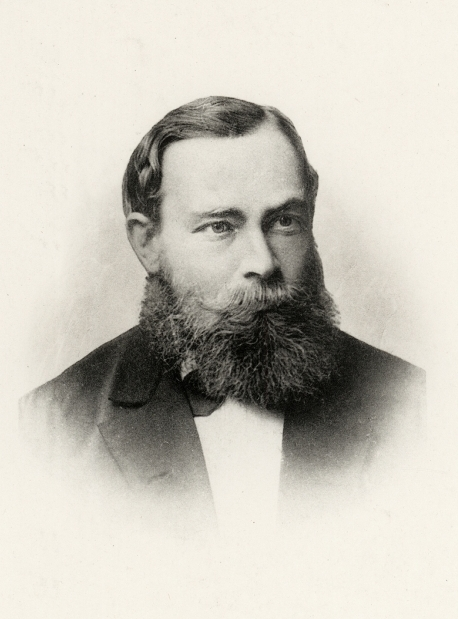
\includegraphics[scale=.45]{graphics/Young-Frege}
	\caption[Young Frege]{Young Frege}
	\label{fig:Frege}
\end{figure}


%\clearpage


\noindent It works in the same way for tables:

\bigskip


{\footnotesize
\noindent \texttt{\textbackslash begin\{table\}[ht!]\\
	\textbackslash centering\\
	\\
	\texttt begin\{tabular\}\{l|l\}\\
	Figure \& Table \textbackslash\textbackslash \\
	\textbackslash hline \\
	test \& test \\
	\textbackslash end\{tabular\}\\
	\\
	\textbackslash caption[Test table]\{Test table\} \\
	\textbackslash end\{table\} }}

\bigskip

\begin{table}[ht!]
	\centering
\begin{tabular}{l|l}
	Figure & Table \\
	\hline
	test & test \\
\end{tabular}
	\caption[Text table]{Test table}
\end{table}


%%%%%%%%%%%%%%%%%%%%%%%%%%%%
%%%%%%%%%%%%%%%%%%%%%%%%%%%%
\section{Examples for different bibliographical entries}
\label{ch:BibEntries}
%%%%%%%%%%%%%%%%%%%%%%%%%%%%


In order to see which information you need in your Bib\TeX\ file for every different entry type (article, book, manuscript, etc.), check the file: \texttt{literature}, or \citet{Freitag&MyP15a}.%
	\footnote{See also \url{https://en.wikipedia.org/wiki/BibTeX}.} %
If you want to see the output for every specific entry type (\fe \texttt{phdthesis} \vs \texttt{book}), take a look at the bibliography of this PDF. This only works in some cases, but you can also try to hold \textsc{ctrl} (or \textsc{cmd} in Mac) and click on the entries' IDs. If it turns underlined and blue, you will be taken to this exact entry in the \texttt{literature} file.


\begin{itemize*}
	\item PhD Thesis: \citet{Abney87a}
	
	\item Article in an edited book: \citet{Ackema15a}
	
	\item Book: \citet{Adger04a}
	
	\item Edited book: \citet{Kertesz&Co19a} %\citet{MyP&Co14b}
	
	\item Article in a journal: \citet{Barwise&Co81a}
	
	\item Article in an online journal or database:
	\citet{Kolb&Co10a}
	
	\item Unpublished work / manuscript: \citet{LeipzigGloss15a}, \citet{MyP17c}
	
	\item Published work without author, using a key, \ie an abbreviation for the citation (this can be used \fe for corpora): \citep{DR17a}
	
	\item Published entry in an encyclopedia (online): \citet{MyP18b}
\end{itemize*}


%%%%%%%%%%%%%%%%%%%%%%%%%%%%
%%%%%%%%%%%%%%%%%%%%%%%%%%%%
\section{Examples for different citation commands with \texttt{natbib}}
\label{ch:CitationCommands}
%%%%%%%%%%%%%%%%%%%%%%%%%%%%


Here are some examples for citation commands. You can find the IDs for every bibliography entry in the file \texttt{literature}, but they are also being suggested as soon as you type in one of the \texttt{\textbackslash cite} commands.


\vspace{.5cm}


\begin{footnotesize}

\begin{tabular}{p{7cm}|p{5.6cm}}
	\textbf{input} & \textbf{output} \\
	\midrule
\verb|\citep{Nolda&Co14a} | & { \citep{Nolda&Co14a}} \\
	
\verb|\citep[cf.][4--5]{Chomsky57a}| & \citep[cf.][4--5]{Chomsky57a} \\
	
 \verb|\citet[cf.][]{Abney87a}| & \citet[cf.][]{Abney87a} \\
	
\verb|\citep[cf.][]{Chomsky70a}| & \citep[cf.][]{Chomsky70a} \\
	
\verb|\citep[56--76]{Heim&Kratzer00a}| & {\citep[56--76]{Heim&Kratzer00a}} \\
	
 \verb|\citealp[56]{Kertesz&Co19a}| & {\citealp[56]{Kertesz&Co19a} }\\
	
 \verb|\citealt[43ff]{Chomsky81b}| &{ \citealt[43ff]{Chomsky81b}} \\
	
\verb|\cf{\fe \citealt{Krifka14a,|  &
	{(cf.\ \fe \citealt{Krifka14a, Chomsky65a};} \\ 
\verb|Chomsky65a,Wiese&Co14a}}| &{\citealt{Wiese&Co14a})} \\
\end{tabular}

\end{footnotesize}


%%%%%%%%%%%%%%%%%%%%%%%%%%%%
%%%%%%%%%%%%%%%%%%%%%%%%%%%%
\section{Abbreviations and indices}
\label{ch:Indices}
\index{index|(} 
%%%%%%%%%%%%%%%%%%%%%%%%%%%%


Some commands are defined in a way that the word used in the command is added to the index of the dissertation. So \fe when \verb|\GB| is used the output in the text is: \GB , and the page in which the term was used is added to the index.  Other commands are connected to the \texttt{acronym} package as well as to the index (see Abbreviations). 


So for instance the command \verb|\GPSG| includes in the first use the whole name and the abbreviation in parentheses cf.\ \GPSG . The next time the the command is used, only the abbreviation is shown, \fe \GPSG . See the definition of both commands (\GB\ and \GPSG ) in the file \texttt{localcommands} and take a look at the section Abbreviations. If you need it, combine in the same fashion all elements in Abbreviations to the index as is done in \texttt{localcommands}.


The pre-defined acronyms in Abbreviations are: 
\begin{multicols}{2}

\begin{itemize*}
\item \ac{acc}, 
\item \ac{ARG-ST}, 
\item \ac{AVM},  
\item \ac{BAG}, 
\item \ac{CP}, 
\item \ac{dat}, 
\item \ac{DTR}, 
\item \ac{EXP}, 
\item \ac{gen}, 
\item \ac{GPSG}, 
\item \ac{HFC}, 
\item \ac{IPA}, 
\item \ac{LEX-DTR}, 
\item \ac{lxgen},  
\item \ac{lxnom}, 
\item \ac{MRS}, 
\item \ac{NP}, 
\item \ac{QP}, 
\item \ac{S}, 
\item \ac{SemP}, 
\item \ac{TAG}, 
\item \ac{TH}. 
\end{itemize*}

\end{multicols}

Own commands are also useful when you don't know yet which spelling you are going to use for a term, \fe the command \verb|\throle| (and \verb|throles| for the plural) can be used to add the term to the index, and, see: one \throle\ and two \throles . If you decide later, that you want to write it with an hyphen, you just need to change the output of the command without looking in the whole document for the terms. In our own commands, there are three commands for indices:

\begin{itemize*}
	\item \verb|\is| has one argument and uses the word(s) written as argument and gives it back in the output as well as including it in the index, \fe \is{argument structure}.
	
	\item \verb|\ist| has one argument and uses the word(s) written as argument giving it back in the output, but in typewriter font, as well as including it in the index (in a normal font), \fe \ist{argument structure}.
	
	\item \verb|ism| has one argument and uses the mathematical symbol written as argument giving it back in the output, as well as including it in the index. The symbols used with this command normally need a math environment, but not inside this command, \fe \verb|\ism{\alpha}| for \ism{\alpha}.
\end{itemize*}


For further information about indices and acronyms, check the documentation of the packages \verb|imakeidx|, \verb|acronym|, and the Wikipedia page for indexing.%
%
\footnote{\url{https://en.wikibooks.org/wiki/LaTeX/Indexing}} %
%


%%%%%%%%%%%%%%%%%%%%%%%%%%%%
%%% END OF SECTION
\index{index|)}
%%%%%%%%%%%%%%%%%%%%%%%%%%%%


%%%%%%%%%%%%%%%%%%%%%%%%%%%%
%%%%%%%%%%%%%%%%%%%%%%%%%%%%
\section{Notes}
\label{ch:Notes}
%%%%%%%%%%%%%%%%%%%%%%%%%%%%


\noindent If you want to write preliminary margin notes, \todo{This note is orange.} you can use the command \texttt{\textbackslash todo} for a note using the package \texttt{\textbackslash todonotes}. Two further commands are defined in the \texttt{localcommands} file. One command for green notes for literature: \texttt{\textbackslash todolit}. \todolit{\citep{Adger04a}} An the other command is for red notes \texttt{\textbackslash todored}. \todored{A red note!}


%%%%%%%%%%%%%%%%%%%%%%%%%%%%
%%%%%%%%%%%%%%%%%%%%%%%%%%%%
\section{Chapter notes}
\label{ch:Chapternotes}
%%%%%%%%%%%%%%%%%%%%%%%%%%%%


A last new command/environment, I found very useful is the environment \verb|chnote|. It works like \texttt{itemize}, but it prints the list in blue. You can use it at the end of your chapters for notes and lists of things you want to add to your chapter later. You will find the definition of this environment in the file \texttt{localcommands}.

\begin{chnote}
	\item Do not forget to read \cite{Barwise&Co81a}.
	\item Add an analysis of postnominal genitive adjuncts.
\end{chnote}


%%%%%%%%%%%%%%%%%%%%%%%%%%%%
%%%%%%%%%%%%%%%%%%%%%%%%%%%%
\section{Helpful literature}
\label{ch:HelpLiterature}
%%%%%%%%%%%%%%%%%%%%%%%%%%%%


When writing your term paper / thesis, you can take a look at the following literature for further help (German explanations are for texts in German):


\begin{itemize*}
	\item \citet{DR17a}: Für Fragen der Rechtschreibung 
	
	\item \citet{MyP17c} oder \citet{Rothstein11a}: Für Fragen bzgl.\ der Fertigstellung von Hausarbeiten
	
	\item \citet{Haspelmath14a}: General style rules for linguistic papers
	
	\item \citet{LeipzigGloss15a}: Glossing rules
	
	\item \citet{Freitag&MyP15a}: Für Fragen bzgl.\ \LaTeX\
	
	\item \citet{Kohm&Co13a}: Für Fragen bzgl.\ der Formatierung mit dem KOMA-Script
	
	\item \citet{Kolb&Co10a}: For questions regarding the syntax of \texttt{gb4e} and \texttt{lsp-gb4eMyP}
	
\end{itemize*}



%%%%%%%%%%%%%%%%%%%%%%%%%%%%
%%%%%%%%%%%%%%%%%%%%%%%%%%%%
%% End of Chapter

%\clearpage



%%%%%%%%%%%%%%%%%%%%%%%%%%%%%%%%%%
%%%             References                      
%%%%%%%%%%%%%%%%%%%%%%%%%%%%%%%%%%

%\begin{singlespace}

%% For two sided documents
\cleardoublepage 

%%% For one sided documents
%\clearpage

\phantomsection %this allows hyperlink in ToC to work
\addcontentsline{toc}{chapter}{References}


%%%% Bibliography style German
%\bibliographystyle{deChicagoMyP}

%%% Bibliography style English
\bibliographystyle{enChicagoMyP}
%\bibliographystyle{unified}

\bibliography{literature}


%%%%%%%%%%%%%%%%%%%%%%%%%%%%%%%%%%
%%%                INDICES
%%%%%%%%%%%%%%%%%%%%%%%%%%%%%%%%%%

%% For two sided documents
\cleardoublepage 

%%% For one-sided documents
%\clearpage

\phantomsection %this allows hyperlink in ToC to work
\addcontentsline{toc}{chapter}{Index} 


\printindex 


%\end{singlespace}


\end{document}